\documentclass[10pt]{beamer}
%\documentclass[10pt,handout]{beamer}

%\usepackage[T1]{CJKutf8}
\usepackage[utf8x]{inputenc}
\usepackage[T1]{fontenc}
%\usepackage{graphicx}
%\usepackage{rotating}
%\usepackage{algpseudocode}

\usepackage{listings}
\usepackage{colortbl}

\newcommand{\includetitlelogo}{
\includegraphics[height=4cm]{titlelogo}}

%\newcommand{\zht}[1]{\begin{CJK}{UTF8}{bsmi}#1\end{CJK}}
\mode<presentation>

\usepackage{xspace}

\usepackage{xcolor}
\hypersetup{urlcolor=blue,colorlinks=true}

\usetheme[english,nologo]{MYplain}
%\usetheme{default}
%\usetheme[english,nologo]{MYplain}
%\usetheme[english,nologo,notitlelogo]{MYplain}


%\renewcommand{\algorithmicrequire}{\textbf{Eingabe:}}
%\renewcommand{\algorithmicensure}{\textbf{Ausgabe:}}

\definecolor{beamer@asblue}{rgb}{.0429,.1718,.4726}


\definecolor{lineblue}{rgb}{0,.156,.559}
\definecolor{linered}{rgb}{.344,0,.07}
\definecolor{cpublue}{rgb}{.457,.563,.828}
\definecolor{alublue}{rgb}{.664,.758,1}
\definecolor{memred}{rgb}{.640,.379,.445}
\definecolor{regred}{rgb}{.879,.676,.711}
\definecolor{cachered}{rgb}{.820,.469,.469}


\newcommand{\F}{\mathbb{F}}
\newcommand{\N}{\mathbb{N}}
\newcommand{\Z}{\mathbb{Z}}
\newcommand{\ggT}{\mathrm{ggT}}
\newcommand{\charac}{\mathrm{char}}
\newcommand{\CO}{\mathcal{O}}

\newcommand{\bl}{\color{beamer@asblue}}
\newcommand{\bk}{\color{black}}
\newcommand{\rd}{\color{red}}
\newcommand{\gr}{\color{green}}
\newcommand{\ord}{\mathrm{ord}}
\newcommand{\divisor}{\mathrm{div}}

\newcommand{\tyrion}{\texttt{tyrion}\xspace}
\newcommand{\arya}{\texttt{arya}\xspace}
\newcommand{\joffrey}{\texttt{joffrey}\xspace}
\newcommand{\hodor}{\texttt{hodor}\xspace}

\newcommand{\mcol}{\multicolumn}


%\usepackage[normalem]{ulem}

\slidecaption{\inserttitle$\quad$--$\quad$\insertsubtitle}

\definecolor{LightCyan}{rgb}{0.88,1,1}
\definecolor{LightRed}{rgb}{1,0.88,0.88}
\newcommand{\LCC}{\cellcolor{LightCyan}}


\usepackage{tikz}
\usetikzlibrary{decorations.pathreplacing}
\usetikzlibrary{shapes,patterns,trees,shadows}
\usetikzlibrary{calc, backgrounds}

\newcommand{\executeiffilenewer}[3]{%
\ifnum\pdfstrcmp{\pdffilemoddate{#1}}%
{\pdffilemoddate{#2}}>0%
{\immediate\write18{#3}}\fi%
}

\newcommand{\includesvg}[2][width=\textwidth]{%
\executeiffilenewer{#2.svg}{#2.pdf}%
  {rsvg-convert -f pdf -o #2.pdf #2.svg}%
\includegraphics[#1]{#2}%
}

\tikzset{
  every overlay node/.style={
    draw=black,fill=white,rounded corners,anchor=center,inner sep=1em
  },
}
% Usage:
% \tikzoverlay at (-1cm,-5cm) {content};
% or
% \tikzoverlay[text width=5cm] at (-1cm,-5cm) {content};
\def\tikzoverlay{%
   \tikz[baseline,overlay]\node[every overlay node]
}%

\def\opac{0.70}


\begin{document}

\title{Network Security}
\subtitle{Anonymous Networks \& Communications}
\date{21 March 2016}
\author{Isis Agora Lovecruft \\
  \small{Core Developer \\
         The Tor Project}
  %\small{<isis@torproject.org>} \\
  %\small{0A6A 58A1 4B59 46AB DE18  E207 A3AD B67A 2CDB 8B35}
}
\institute{Raboud University, The Netherlands}

\frame[plain]{\titlepage}

\begin{frame}
  \frametitle{About}
  \begin{itemize}
    \item Disclaimer: IANACSNAC
      \tiny (I Am Neither A Computer Scientist Nor A Cryptographer) \normalsize
    \item<2-> Studied Physics, specialising in HEP Theory, and English Literature,
      specialising in Feminist Critical Theory
    \item<3-> Developer for The Tor Project since 2010
    \item<4-> Previous projects include design and development of the Open
      Observatory of Network Interference (OONI), an open-source,
      open-methodology platform for large-scale tests for online censorship and
      other global network anomalies.
    \item<5-> Current work includes development on Tor Bridges and
      Pluggable Transports, development on backend infrastructure
      within the Tor Network, distribution of Tor Bridges, Tor
      circuit-level crypto and path manipulation.
    \item<6-> More information: \url{https://fyb.patternsinthevoid.net} \\
      Including asciiart and My Little Ponies which bounce around in your
      browser (if you trust me enough to enable Javascript). \\
      It also has useful things: technical blogposts, project ideas and updates,
      my public keys and fingerprints, and, of course, links to all my code.
  \end{itemize}
\end{frame}

\begin{frame}
  \frametitle{Why should you care about privacy?}
  \begin{quotation}
    ``There is an entire genre of YouTube videos devoted to an experience which
    I'm certain that everyone in this room has had. It entails an individual,
    who, thinking they're alone, engages in some expressive behaviour -- wild
    singing, girating dancing, some mild sexual activity -- only to discover
    that, in fact, they are not alone, that there's a person watching and
    lurking, the discovery of which causes them to immediately cease what
    they're doing in horror. The sense of shame and humiliation in their face is
    palpable: it's the sense of `this is something I'm willing to do only if no
    one else is watching.'  This is the crux of the work on which I have been
    singularly focused for the sixteen months: the question of why privacy matters.'' \\
    \hfill{\raggedright---Glenn Greenwald,
      \href{https://www.youtube.com/watch?v=pcSlowAhvUk}{TED Talk}, October 2014}
  \end{quotation}
\end{frame}


\begin{frame}
  \frametitle{But I have nothing to hide…}
  \begin{quotation}
    ``Arguing that you don't care about the right to privacy because you have
    nothing to hide is no different than saying you don't care about free speech
    because you have nothing to say'' \\
    \hfill{\raggedright---Ed Snowden,
      \href{https://www.reddit.com/r/IAmA/comments/36ru89/just_days_left_to_kill_mass_surveillance_under/crglgh2}{Reddit AMA}, 21 May 2015}
  \end{quotation}
\end{frame}
  

\begin{frame}
  \frametitle{Privacy is necessary for all other rights}

  \begin{block}{Even if you don't care about your own right to privacy $\dots$}
  \begin{itemize}
    \item<1-> $\dots$ it's incredibly antisocial to claim that the right to privacy as
      a whole should be reliquished, that others should also be expected to have
      nothing to hide.
    \item<2-> $\dots$ it's saying, ``I don't care about \emph{your} right to
      privacy; I don't care about your rights to freedom of expression and
      freedom of speech. I don't care about anyone different to me.''
  \end{itemize}
  \end{block}

  \uncover<3->{
    \begin{quotation}
      ``Privacy is the right from which all others are derived. Privacy is the
      fountainhead of individuality.  Without privacy, there is only the
      collective, there is only society, there is only influence from groups, from
      large powers, that shape every person to bring them
      into that fold and to make them all alike.'' \\
      \hfill{\raggedright---Ed Snowden,
        \href{https://www.youtube.com/watch?v=Ha0H4B_tYnU}{CIJ Logan Symposium}, 12 March 2016}
    \end{quotation}
  }
\end{frame}


\begin{frame}
  \frametitle{Privacy is necessary because laws and norms change}

  \begin{block}{So let's assume $\dots$}
  \begin{itemize}
    \item $\dots$ You have nothing to hide.
    \item<2-> $\dots$ You have never done anything wrong.
    \item<3-> $\dots$ You have never done anything illegal.
    \item<4-> $\dots$ You don't care about anyone else's rights.
    \item<5-> \textbf{You should still care about your own right to privacy,
      because laws and societal norms change, or may be interpreted
      differently over time.}
  \end{itemize}
  \end{block}

  \uncover<6->{
  In the United States, it's not only unknowable \emph{which} laws
  might apply: it's actually unknowable \emph{how many} laws might
  apply at a given place and time -- let alone how they may be
  interpreted by a particular court.}
\end{frame}


\begin{frame}
  \frametitle{Privacy is necessary because laws and norms change}
  \begin{quotation}
    ``Estimates of the current size and body of the [United States]
    federal criminal law vary. It has been reported that the
    Congressional Research Service cannot even count the current
    number of federal crimes.  And these laws are scattered in over fifty
    titles of the United States Code, encompassing roughly 27,000
    pages. Worse yet, the statutory code sections often incorporate,
    by reference, the provisions and sanctions of administrative
    regulations promulgated by various regulatory agencies. Estimates
    of how many such regulations exist are even less well settled, but
    the American Bar Association thinks there are nearly 10,000.'' \\
    \hfill{\raggedright---James Duane, Regent Law Professor, in a
      \href{https://www.youtube.com/watch?v=d-7o9xYp7eE}{lecture}
      entitled ``Don't Talk to Police'', May 2012}
  \end{quotation}
\end{frame}


\begin{frame}
  \frametitle{Privacy is necessary for scientific progress}

  Privacy is essential for continued open progression of scientific
  understanding and human knowledge.


  \begin{block}{From Juice Rap News, ``Big Brother is WWWatching You'':}
  \begin{quotation}
    \footnotesize
    We're told we need safety; which is precious, yes, \\
    But can a society that can enforce \emph{all} it's laws ever progress? \\
    Hindsight shows that many figures guilty of ``thoughtcrime'' \\
    Turned out to be luminaries and heroes, before their time. \\
    {[}images of Martin Luther King, Galileo, Huey P. Newton, others{]} \\
    But if the surveillance state had reigned then, in this form~and~design, \\
    Just think of all the progress we may've been denied: \\
    Could lobbies for women's or gay rights have appeared and~thrived? \\
    Would revolutionary ideals have materialised? \\
    Would science have pioneered or even survived, \\
    If every word had been monitored by thought police and spies?
    \normalsize
  \end{quotation}
  \small\url{https://youtu.be/o66FUc61MvU}\normalsize
  \end{block}

  % Show video
\end{frame}


\begin{frame}
  \frametitle{But most web traffic now is encrypted, right?}
  \uncover<2->
  {
    \begin{center}
      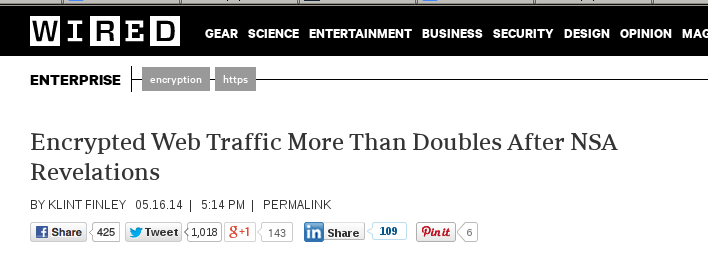
\includegraphics[width=11cm]{webencrypt}
    \end{center}
  }
\end{frame}

\addtocounter{framenumber}{-1}
\begin{frame}
  \frametitle{Actually, no, everything is not encrypted, not really}
  From the article:\\[.3cm]

  \begin{quotation}
    ``Early last year–before the Snowden revelations–encrypted traffic accounted for 2.29 percent of all peak hour traffic in North America, 
    according to Sandvine’s report. Now, it spans 3.8 percent. But that’s a small jump compared to other parts of the world. 
    In Europe, encrypted traffic went from 1.47 percent to 6.10 percent, and in Latin America, it increased from 1.8 percent to 10.37 percent.''\\
    \hfill{\raggedright---Klint Finley on wired.com, May 16, 2014} %XXX: make look nice
  \end{quotation}
\end{frame}

\begin{frame}
  \frametitle{$\dots$update from 2015}
  \begin{center}
    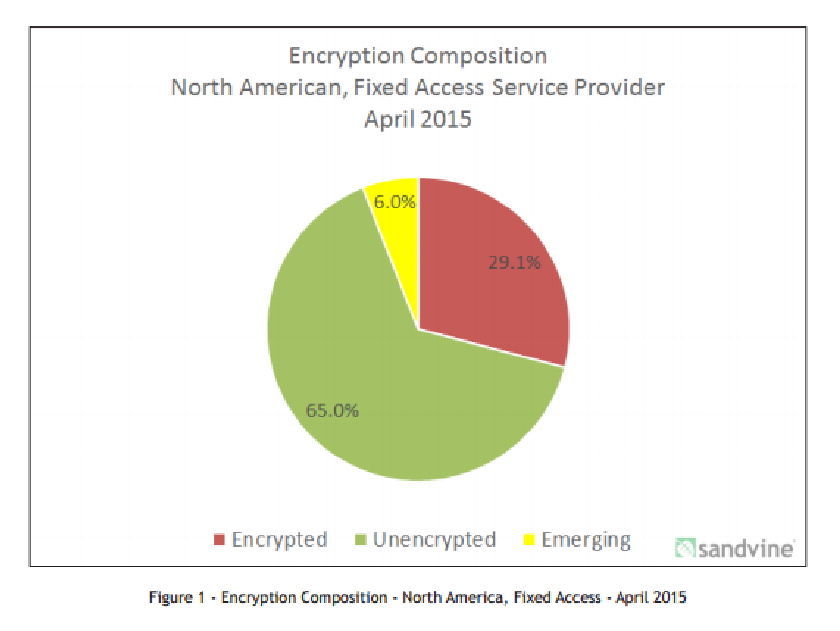
\includegraphics[width=10cm]{webencrypt2015}
  \end{center}
\end{frame}

\begin{frame}
  \frametitle{$\dots$estimated for 2016}
  %\only<1>{
  %\begin{center}
  %  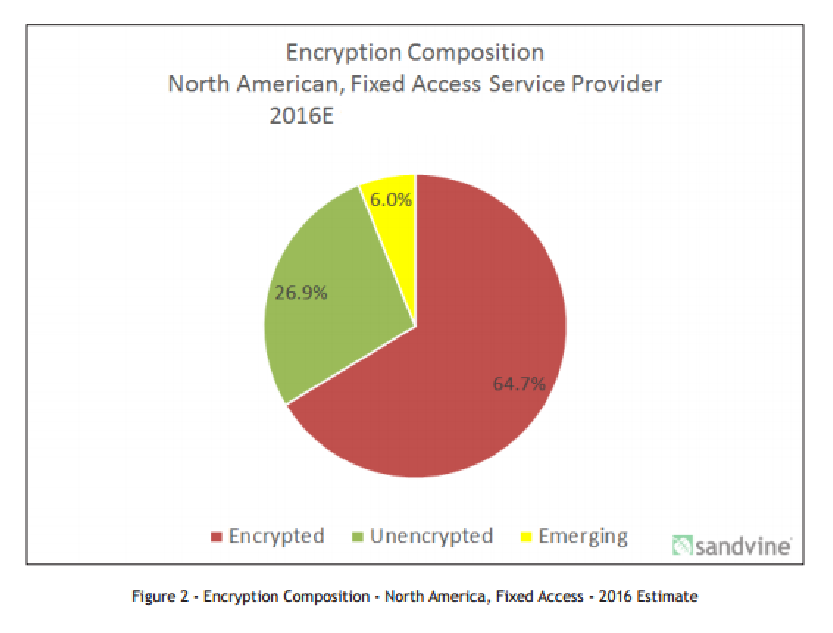
\includegraphics[width=10cm]{webencrypt2016edit}
  %\end{center}} 
  %\only<2>{
  \begin{center}
    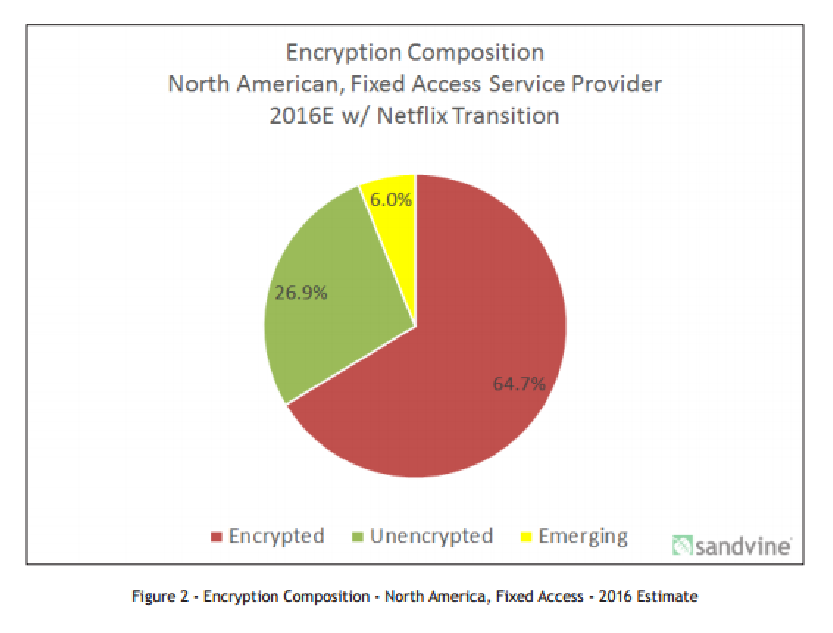
\includegraphics[width=10cm]{webencrypt2016}
  \end{center}
  %} 
\end{frame}


\begin{frame}
  \frametitle{Okay, but! if everything were encrypted $\dots$}

  \begin{block}{Imagine a world in which $\dots$}
  \begin{itemize}
    \item $\dots$ all Internet traffic is encrypted and authenticated,
    \item<2-> $\dots$ emails are all signed and encrypted end-to-end,
    \item<3-> $\dots$ everybody is using ciphersuites that offer high security,
    \item<5-> $\dots$ crypto implementations are correct, secure, side-channel
      resistant, formally verified, and expose impossible-to-misuse APIs to
      applications developers,
    \item<6-> $\dots$ applied cryptographers have trouble finding jobs.
  \end{itemize}
  \end{block}

  \uncover<7->{\textbf{They still get the ``metadata''.}}
\end{frame}


\begin{frame}
  \frametitle{What even is this ``metadata'' stuff?}

  \uncover<2->{
  \begin{block}{EU's Data Retention Directive}
    \scriptsize (Annulled in 2014, when the European Parliament found blanket
    data rentention of unsuspicious persons to generally violate the EU Charter
    of Fundamental Rights.)}\normalsize

    \uncover<3->{ \small
    \emph{``Member States shall ensure that the categories of data specified in
      Article 5 are retained for periods of not less than six months and not
      more than two years from the date of the communication.''}\normalsize}

    \uncover<4-> { From Article 5: \\
      \begin{itemize}
        \item<4-> data necessary to trace and identify both the source and
          destination of a communication
        \item<5-> data necessary to identify the date, time and duration of a communication
        \item<6-> data necessary to identify the type of communication
        \item<7-> data necessary to identify users' communication equipment or what purports to be their equipment
        \item<8-> data necessary to identify the location of mobile communication equipment
      \end{itemize}
    }
  \end{block}

  \uncover<9->{\textbf{Encrypting and authenticating content doesn't prevent any of this!}}
\end{frame}


\begin{frame}
  \frametitle{But ``it's just metadata''!}
  \begin{quotation}
    ``Metadata absolutely tells you everything about somebody’s life. 
    If you have enough metadata you don’t really need content$\dots$ 
    [It’s] sort of embarrassing how predictable we are as human beings.'' \\
    \hfill---Stewart Baker, former general counsel of the NSA\\[1cm]
  \end{quotation}

  \uncover<2->
  {
    \begin{quotation}
      ``Metadata is our context. And that can reveal far more about us than the
      words we speak. Context yields insights into who we are and the implicit,
      hidden relationships between us.'' \\
      \hfill---Matt Blaze
      \href{http://www.wired.com/2013/06/phew-it-was-just-metadata-not-think-again/}{on
        wired.com}, June 2013
    \end{quotation}
  }

  \uncover<3->
  {
    \begin{quotation}
    ``We kill people based on metadata.''\\
    \hfill---Michael Hayden, former director of the NSA and the CIA
    \end{quotation}
  }
\end{frame}


\begin{frame}
  \frametitle{Is ``metadata'' all an attacker gets?}
  \begin{itemize}
    \item Common assumption: this ``metadata'' only includes who is talking to
      whom, or which website is being requested, but we assume ``metadata'' does
      include any information about the content.
    \item Example, interview with Jimmy Wales (Wikipedia founder):\\[2mm]
      ``\emph{\textbf{You've said that you're going to start encrypting communications on Wikipedia as a result$\dots$}\\[3mm]
      We have done. It's not completely finished yet but the only thing that GCHQ, hopefully, 
      can see is that you're looking at Wikipedia. They can't see which article you're reading. 
    It's not the government's business to know what everybody is reading.''}
  \item<2-> Small experiment: $10$ Wikipedia pages, load one at random through HTTPS
  \item<2-> Attacker sniffs the network, tries to figure out which one
  \item<5-> In this (contrived, closed-world) scenario, it's not that hard: 
    \begin{itemize}
      \item $10$ webpages have different amount of pictures
      \item $10$ webpages have different (length of) URLs to pictures
      \item Attacker can count bytes of requests to image server
      \item<6-> This is not the only thing an attacker sees: number of requests,
        timings, delays, responses$\dots$
    \end{itemize}
  \end{itemize}

\end{frame}


\begin{frame}
  \frametitle{What can we do to protect our privacy?}

  If encryption alone is not enough, what more can we do to protect our data?

  \uncover<2->{
  \begin{block}{Report of the Special Rapporteur on the promotion and protection
      of the right to freedom of opinion and expression:}
    \begin{quotation}
      ``States should promote strong encryption and anonymity. National laws
      should recognize that individuals are free to protect the privacy of their
      digital communications by using encryption technology and tools that allow
      anonymity online. Legislation and regulations protecting human rights
      defenders and journalists should also include provisions enabling access
      and providing support to use the technologies to secure their
      communications.'' \\
      \hfill{\raggedright---David Kaye,
        \href{www.ohchr.org/EN/HRBodies/HRC/RegularSessions/Session29/Documents/A.HRC.29.32_AEV.doc}{Report},
        May 2015}
    \end{quotation}
  \end{block}}
\end{frame}


\begin{frame}
  \frametitle{Terminology: Anonymity Set}

  \begin{itemize}
    \item \textbf{Anonymity Set.} ``To enable the anonymity of a subject, there always
    has to be an appropriate set of subjects with potentially the same
    attributes.  Anonymity is thus defined as the state of being not identiable
    within a set of subjects, the anonymity set.

    The anonymity set is the set of all possible subjects.  With respect to
    acting entities, the anonymity set consists of the subjects who might cause
    an action.  With respect to addressees, the anonymity set consists of the
    subjects who might be addressed.  Both anonymity sets may be disjoint, be
    the same, or they may overlap.  The anonymity sets may vary over time.''
  \end{itemize}
\end{frame}


\begin{frame}
  \frametitle{Terminology: Unlinkability}

  \begin{itemize}
    \item<2-> \textbf{Absolute Unlinkability.} ``Absolute unlinkability ensures that a user
      may make multiple uses of resources or services without others being able to
      link these uses together.  [...]  Unlinkability requires that users and/or
      subjects are unable to determine whether the same user caused certain specic
      operations in the system.''
    \item<3-> \textbf{Relative Unlinkability.} ``Unlinkability of two or more items of
      interest (e.g., subjects, messages, events, actions, ...)  means that within
      the system (comprising these and possibly other items), from the attacker's
      perspective, these items of interest are no more and no less related after
      her observation than they were related concerning her a-priori knowledge.''
  \end{itemize}
\end{frame}

\begin{frame}
  \frametitle{Trusted and Semi-Trusted relays}

  \begin{block}{There are two broad categories for designs of anonymous
      communications networks:}
    \begin{itemize}
    \item<2-> Those that use trusted relays, i.e. the privacy/anonymity guarantees
      of the system rely on one centralised node.
    \item<3-> Those that use semi-trusted relays, i.e. compromise of any one node
      in the network should not degrade the privacy/anonymity of the user.
    \end{itemize}
  \end{block}
\end{frame}


\begin{frame}
  \frametitle{Trusted-Relays Systems: Email}

  \begin{block}{Danezis, George, and Claudia Diaz. \\
      A survey of anonymous communication channels. \\
      Technical Report MSR-TR-2008-35, Microsoft Research, 2008.}
  \begin{quotation}
    ``Johan Helsingius started running a trusted mail relay, anon.penet.fi,
    providing anonymous and pseudonymous email accounts in 1993.  The
    technical principle behind the service was a table of correspondences
    between real email addresses and pseudonymous addresses, kept by the
    server.  Email to a pseudonym would be forwarded to the real user.  Email
    from a pseudonym was stripped of all identifying information and forwarded
    to the recipient.  While users receiving or sending email to a pseudonym
    would not be able to nd out the real email address of their anonymous
    correspondent, it would be trivial for a local passive attacker or the
    service itself to uncover the correspondence by correlating the timing of
    incoming and outgoing email traffic.''
  \end{quotation}
  \end{block}
\end{frame}


\begin{frame}
  \frametitle{Trusted-Relay Systems: IPsec Tunneling}

  \resizebox{\textwidth}{!}{%
    \begin{tikzpicture}
      \path[use as bounding box]
      %  \path[draw] 
      (-1.5,-3) rectangle (16.25, 3);
      \coordinate (pc1c) at (0,0);
      \node[anchor=south] (pc1c-1) at ([yshift=0.5cm]pc1c.north) {\includesvg[width=3cm]{fig/pc}};
      \node[anchor=north] (pc1c-2) at ([yshift=-0.5cm]pc1c.south) {\includesvg[width=3cm]{fig/pc}};
      \node[anchor=center] at (pc1c) {local network};
      \node[anchor=west] (s1) at ([xshift=3cm]pc1c.east) {\includesvg[width=1.5cm]{fig/server}};
      \node[anchor=north]  at (s1.south) {gateway};
      \node [cloud, draw,cloud puffs=10,cloud puff arc=120, aspect=2, anchor=west, align=center,
      text width=2cm]
      (cloud) at ([xshift=5.75cm]pc1c.east) {Internet};
      \node[anchor=west] (s2) at ([xshift=1cm]cloud.east) {\includesvg[width=1.5cm]{fig/server}};
      \node[anchor=north] at (s2.south) {gateway};
      \node (pc2) at ([xshift=3cm]s2.east) {};
      \node[anchor=center]  at (pc2) {local network};
      \node[anchor=south] (pc2-1) at ([yshift=0.5cm]pc2.north) {\includesvg[width=3cm]{fig/pc}};
      \node[anchor=north] (pc2-2) at ([yshift=-0.5cm]pc2.south) {\includesvg[width=3cm]{fig/pc}};
      \draw[<->, thick] (pc1c-1) -- (s1);
      \draw[<->, thick] (pc1c-2) -- (s1);
      \draw[<-, thick] (s1) -- (cloud);
      \draw[->, thick] (cloud) -- (s2);
      \draw[<->, thick] (s2) -- (pc2-1);
      \draw[<->, thick] (s2) -- (pc2-2);
      \node[double arrow, draw, text width=4.5cm, align=center, fill=white] 
      at ([yshift=0.75cm]$ (s1.east) !.5! (s2.west) $) {tunnel mode};
    \end{tikzpicture}%
  }
  \begin{itemize}
    \item Everything between the gateways has the \emph{gateways' addresses}
    \item Nodes behind the gateways are indistinguishable
    \item \href{https://tools.ietf.org/rfc/rfc2406.txt}{RFC 2406} calls this ``limited traffic flow confidentiality''
    \item<2-> Problem 1: Does not help against state-level attacker who can request gateway's logfiles
    \item<3-> Problem 2: Potentially small anonymity set
  \end{itemize}

\end{frame}


\begin{frame}
  \frametitle{Trusted-Relay Systems: Anonymizing proxies}
  \begin{itemize}
    \item Somewhat similar idea (without crypto): use a proxy server
    \item Typically: application-specific proxies (e.g., HTTP proxies) or
      generic request-based proxies (e.g. SOCKS proxies)
    \item Requests to websites come from proxy 
    \item All users behind the proxy are indistinguishable
    \item Various problems:
      \begin{enumerate}
        \item Single point of failure against state-level attackers
        \item<2-> Proxy somewhere in the Internet: easy to correlate ingoing/outgoing traffic
        \item<3-> No crypto protection from the user to the proxy
      \end{enumerate}
    \item<4-> Can add crypto to the proxy (e.g., OpenVPN Service)
    \item<4-> That still does not solve problems 1 and 2, that is: Virtual
      Private Networks increase user privacy but do not substantially improve
      anonymity. Additional problems are added: in the case of VPNs, the VPN
      fails open, meaning that when the tunnel to the private network breaks
      down, user traffic goes out in the clear.
  \end{itemize}
\end{frame}


\begin{frame}
  \frametitle{Trusted-Relay Systems}

  We can see from the previous examples that designs which place ultimate trust
  in any single node in the network cannot provide any strong guarantees to
  anonymity, because these single points of failure can be exploited (legally or
  otherwise) to deanonymise users.
\end{frame}


% \begin{frame}
%   \frametitle{Why is privacy important?}
%   \begin{itemize}
%     \item Personal anecdote about my mom writing a Perl script to
%       block DNS requests containing the substring ``music''.
%     \item 10-year-old me's solution: Go to search page for
%       http://latimes.com, use the embedded iframe of results (on
%       http://google.stanford.edu) to find BBS page containing the
%       classical piano sheet music I wanted, and load the sheet music
%       within the iframe.
%   \end{itemize}
% \end{frame}


\begin{frame}
  \frametitle{Trusted-Relay Systems: Mix Networks}

  Mix networks are routing protocols that create hard-to-trace communications by
  using a chain of nodes, known as mixes, which receive messages from multiple
  senders, shuffle them in some manner, and send them to the next destination.

  \uncover<2->{
  \begin{block}{Chaum's Original Mix Networks}
  \begin{itemize}
    \item<2-> Idea for anonymous electronic mail by David Chaum, in 1981.
    \item<3-> There should exist some well-known public key for each mix.
    \item<4-> Messages are split up into blocks and encrypted to the mix's
      public key.
      % The first few blocks conceptually contain some ``headers'',
      % which are stripped at each hop, then some random cruft is added to the end
      % of each message.
    \item<5-> Each mix only knows the nodes immediately before and after it,
      making the network resistant to malicious mix nodes.
    \item<6-> Supposed to achieve \emph{bitwise unlinkability} between the
      source of the message and the destination, making it difficult for an
      adversary to trace end-to-end communications end-to-end.
    \item<7-> Message shuffling in order to achieve unlinkability.
  \end{itemize}
  \end{block}}
\end{frame}


\begin{frame}
  \frametitle{Trusted-Relay Systems: Mix Networks}

  \begin{block}{Problems with Chaum's Original Mix Network Scheme}
    \begin{itemize}
      \item Pfitzmann and Pfitzmann (1990) demonstrated that Chaum's original
        work did not acheive the desired unlinkability property.
      \item<2-> \emph{Tagging attacks} are possible: each encrypted message block,
        using RSA, is not dependent on those before or after it, and thus can be
        substituted or reused.
        % XXX is there a name for the attack where you trick someone into signing
        % by asking them to decrypt?
      \item<3-> Most of Chaum's work was done in the late 1970s.
        Unsurprisingly, it used RSA in ways now known to be unsafe, i.e. without
        padding, applying the modular exponations directly to messages.
      \item<4-> Because the RSA operation was applied directly, an adversary
        could trick a mix into signing a message by applying the decryption
        operation.
        \begin{itemize}
          \item<5-> This attack could be further hidden from the mix by applying
            a signature blinding technique.
          \item<6-> To be fair, Chaum invented RSA blind signing two years later, in
            1983.
        \end{itemize}
    \end{itemize}
  \end{block}
\end{frame}


\begin{frame}
  \frametitle{Trusted-Relay Systems: Mix Networks}

  \begin{block}{Type II Anonymous Remailers: Sending a message}
  \begin{itemize}
    \item Assume that Alice wants to anonymously send message $M$ to Bob
    \item<2-> Uses intermediate computer called \emph{mix} and public keys
      \begin{itemize}
        \item $K_B$ of Bob, and
        \item $K_M$ of the mix
      \end{itemize}
    \item<3-> Sends to mix: $K_M(R_1,K_B(R_0,M))$ for random $R_0, R_1$
    \item<4-> Mix collects many such mails, decrypts to $K_B(R_0,M)$
    \item<5-> Sends mails in lexicographic order to receivers
    \item<5-> Receiver Bob decrypts and obtains $M$
    \item<6-> Achieves anonymity if encrypted messages are indistinguishable
    \item<6-> Very important: never repeat input and output!
    \item<6-> No protection against \emph{tagging attacks} and \emph{replay attacks}
    \item<6-> Has high communication latency (the mix should wait for enough
      messages to be within the mixing pool so as to provide some sufficient
      anonymity set for the clients)
  \end{itemize}
  \end{block}
\end{frame}


\begin{frame}
  \frametitle{Trusted-Relay Systems: Mix Networks}

  \begin{block}{Type II Anonymous Remailers: Return addresses}
  \begin{itemize}
    \item Need a way for Bob to reply without revealing Alice's address/identity
    \item<2-> Alice includes a return address her message encrypted to Bob:
      $$K_M(R_1,A_X),K_X$$
    \item<2-> $R_1, K_X$ are random one-time symmetric keys
    \item<2-> $A_X$ is Alice's real address
    \item<3-> Bob can send response $M$ as
      $$K_M(R_1,A_X),K_X(R_0,M)$$
    \item<4-> Mix receives and recovers $R_1, A_X$, sends to Alice
      $$R_1(K_X(R_0,M))$$
    \item<5-> Only Alice can decrypt, because only she knows both $K_X$ and $R_1$
  \end{itemize}
  \end{block}
\end{frame}


\begin{frame}
  \frametitle{Mix Network Designs: Cascading Mixes}

  Chaum noted that relying on only one mix is not resilient against malicious
  nodes, so the function of mixing should distributed.  Mixes can be chained to
  ensure that, even if just one of them remains honest, some anonymity is
  provided.

  \uncover<2->{
  First proposed way to chain mixes together is called \emph{cascade mixing},
  and uses all nodes in the network, in a specific order:

  \begin{center}
    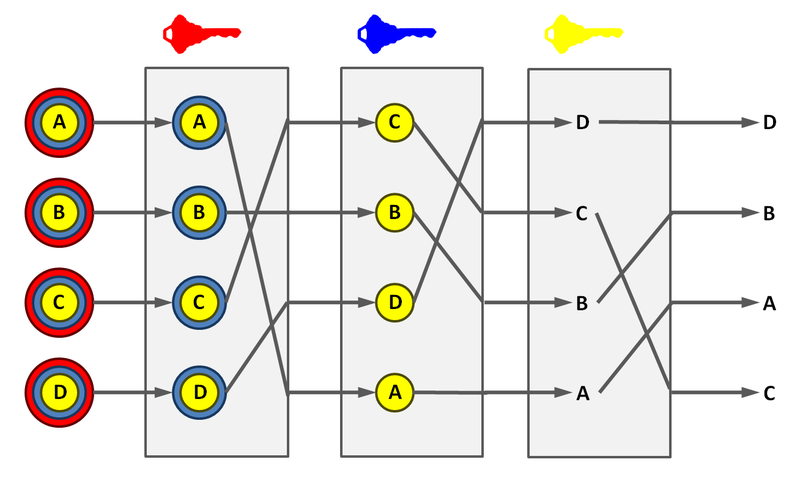
\includegraphics[width=10cm]{cascading}
  \end{center}}
\end{frame}


\begin{frame}
  \frametitle{Mix Network Designs: Mix Networks}

  The second way is to allow users to arbitrarily select which mixes their
  message will pass through, and is what is now generally referred to as a
  \emph{mix network}.

  \uncover<2->{
  \begin{block}{This design has some problems:}
    \begin{itemize}
    \item Berthold, Pfitzmann, and Standtke (2000) argue that mix networks do
      not offer some properties that cascades offer.
    \item<3-> They illustrate a number of attacks to show that, if \emph{only one}
      mix is honest in the network, the anonymity of the messages going
      through it can be compromised.
    \item<4-> These attacks rely on compromised mixes which exploit some
      knowledge of their position in the chain $\dots$
    \item<5-> $\dots$ or multiple messages using the same sequence of mixes
      through the network.
    \end{itemize}
  \end{block}}
\end{frame}


\begin{frame}
  \frametitle{Trusted-Relay Systems: Mix Networks}

  \begin{block}{Type II Anonymous Remailers: Mixmaster}
    \begin{itemize}
    \item Mixmaster was created in 1995 and has some differences to previous
      Type II anonymous remailers.
    \item<2-> Supports only \emph{forward path}, i.e. sender, anonymity.
    \item<3-> Messages are bitwise unlinkable via hybrid RSA and EDE 3DES.
    \item<4-> Messages can be divided in smaller chunks and sent via independent
      paths.  If all parts end up at a common mix, then reconstruction happens
      transparently.
    \item<5-> v2: The integrity of the RSA-encrypted header is protected by a
      hash, making tagging attacks on the header impossible.
    \item<6-> v3: The appended noise is deterministically generated using a
      secret shared between the mix and the sender of the message, and this is included in
      the header.
      \begin{itemize}
      \item<7-> Allows an additional header containing a hash of the entire message.
      \item<8-> Makes replies impossible to construct: the body of the reply
        would not be known to the creator of the anonymous address block, so it
        isn't possible to compute in the hash.
      \end{itemize}
  \end{itemize}
  \end{block}
\end{frame}


\begin{frame}
  \frametitle{Mix Nets vs. Anonymizing proxies}
  \begin{columns}[t]
    \column{.5\textwidth}
    \begin{block}{Mix Nets}
      {\gr $\mathbf{+}$} No single point of failure (with cascading)\\
      {\gr $\mathbf{+}$} Inbound/output-traffic analysis does not deanonymise\\
      {\gr $\mathbf{+}$} Generally good anonymity guarantees\\
      \uncover<2->{
        {\rd $\mathbf{-}$} Slow public-key cryptography (at least in vanilla mix nets)\\
        {\rd $\mathbf{-}$} High latency
      }
    \end{block}
    \column{.5\textwidth}
    \uncover<3->
    {
    \begin{block}{Anon. Proxies}
      {\gr $\mathbf{+}$} Low latency\\
      {\gr $\mathbf{+}$} No overhead from slow crypto\\
      \uncover<4->
        {
      {\rd $\mathbf{-}$} Single point of failure\\
      {\rd $\mathbf{-}$} Inbound/output-traffic analysis deanonymises\\
      {\rd $\mathbf{-}$} No strong anonymity guarantees
        }
    \end{block}
    }
  \end{columns}
  \vspace*{4mm}
  \uncover<5->
  {
    \noindent \textbf{Idea of Onion Routing: Combine advantages:}
  \begin{itemize}
    \item Use cascade of ``proxies'', called \emph{Tor relays} or \emph{Tor nodes}
    \item Use asymmetric crypto for establishing an authenticated and encrypted
      channel, then use fast symmetric crypto.
  \end{itemize}
  }
\end{frame}


\begin{frame}
  \frametitle{Onion Routing and Tor}

  \pgfdeclarelayer{l0}
  \pgfdeclarelayer{l1}
  \pgfdeclarelayer{l2}
  \pgfsetlayers{l0,l1,l2,main}

  \begin{columns}

    \column{.4\textwidth}
    \begin{tikzpicture}
      \path[use as bounding box]
      %  \path[draw] 
      (-6.6,-3.2) rectangle (14.1, 2.2);

      \tikzstyle{box}=[align=center, 
        anchor=north east, minimum height=1cm,
        %text height=1.5ex, text depth=.25ex,
      postaction={draw,thin},line width=0cm];

      \only<3->{
      \node[box, minimum width = 3.5cm, minimum height = 2cm, fill=gray!40]
      (dest) at (-2,-2)  {Request};

%      \node[box, minimum width=3.5cm, minimum height=4cm, anchor=west, fill=green!40]
%      (tcps) at (tcph.east) {IP Packet};

%      \draw[line width=1pt] (tcph.south west) rectangle (tcps.north east);
      }
      \only<4->
      {
      \begin{pgfonlayer}{l2}
        \node[box, minimum height=3.5cm, minimum width=4cm, anchor=center, fill=yellow!80] (exit)
        at ([xshift=10mm]$ (dest.north west) !.2! (dest.south east) $) {};
        \node[anchor=north] at (exit.north) {Encrypted with $KF_{R_3}$};
        \node[anchor=north] at ([yshift=-8mm] exit.north) {to \texttt{theintercept.com}};
      \end{pgfonlayer}
      }

      \only<5->
      {
      \begin{pgfonlayer}{l1}
        \node[box, minimum height=5cm, minimum width=4.5cm, anchor=center, fill=blue!60] (guard)
        at ([xshift=7mm]$ (exit.north west) !.3! (exit.south east) $) {};
        \node[anchor=north] at (guard.north) {Encrypted with $KF_{R_2}$};
        \node[anchor=north] at ([yshift=-8mm] guard.north) {to $R_3$};
      \end{pgfonlayer}
    }

      \only<6->
      {
      \begin{pgfonlayer}{l0}
        \node[box, minimum height=6.5cm, minimum width=5cm, anchor=center, fill=red!60] (entry)
        at ([xshift=4mm]$ (guard.north west) !.4! (guard.south east) $) {};
        \node[anchor=north] at (entry.north) {Encrypted with $KF_{R_1}$};
        \node[anchor=north] at ([yshift=-8mm] entry.north) {to $R_2$};
      \end{pgfonlayer}
    }


    \end{tikzpicture}%

    \column{.6\textwidth}
    \begin{itemize}
      \item Assume user has public keys for all relays.
      \item<2-> Use relay public keys to setup an authenticated and encrypted
        channel, which is used to establish symmetric keypairs for the
        \emph{forward} and \emph{reverse paths}:
        \begin{itemize}
          \item Entry relay $R_1$ (keys $KB_{R_1}$, $KF_{R_1}$)
          \item Middle relay $R_2$ (keys $KB_{R_2}$, $KF_{R_2}$)
          \item Exit relay $R_3$ (keys $KB_{R_3}$, $KF_{R_3}$)
        \end{itemize}
      \item<3-> Wants to anonymously send request to \texttt{theintercept.com}
      \item<4-> Prepares packet as follows:
        \begin{itemize}
          \item<4-> Write dest. \texttt{theintercept.com}, encrypt with $KF_{R_3}$
          \item<5-> Write dest. $R_3$ encrypt with $KF_{R_2}$
          \item<6-> Write dest. $R_2$ encrypt with $KF_{R_1}$
        \end{itemize}
      \item<7-> Send this packet to $R_1$
    \end{itemize}
  \end{columns}
\end{frame}



\addtocounter{framenumber}{-1}
\begin{frame}
  \frametitle{Onion Routing and Tor}

  \pgfdeclarelayer{l0}
  \pgfdeclarelayer{l1}
  \pgfdeclarelayer{l2}
  \pgfsetlayers{l0,l1,l2,main}

  \begin{columns}

    \column{.4\textwidth}
    \begin{tikzpicture}
      \path[use as bounding box]
      %  \path[draw] 
      (-6.6,-3.2) rectangle (14.1, 2.2);

      \tikzstyle{box}=[align=center, 
        anchor=north east, minimum height=1cm,
        %text height=1.5ex, text depth=.25ex,
      postaction={draw,thin},line width=0cm];

      \node[box, minimum width = 3.5cm, minimum height = 2cm, fill=gray!40] (dest) at (-2,-2)  {Request};

      \only<1-5>
      {
      \begin{pgfonlayer}{l2}
        \node[box, minimum height=3.5cm, minimum width=4cm, anchor=center, fill=yellow!80] (exit)
        at ([xshift=10mm]$ (dest.north west) !.2! (dest.south east) $) {};
        \node[anchor=north] at (exit.north) {Encrypted with $KF_{R_3}$};
      \end{pgfonlayer}
      }
      
      \only<1-6>
      {
        \node[anchor=north] at ([yshift=-8mm] exit.north) {to \texttt{theintercept.com}};
      }


      \only<1-3>
      {
      \begin{pgfonlayer}{l1}
        \node[box, minimum height=5cm, minimum width=4.5cm, anchor=center, fill=blue!60] (guard)
        at ([xshift=7mm]$ (exit.north west) !.3! (exit.south east) $) {};
        \node[anchor=north] at (guard.north) {Encrypted with $KF_{R_2}$};
      \end{pgfonlayer}
      }
        
      \only<1-4>
      {
      \node[anchor=north] at ([yshift=-8mm] guard.north) {to $R_3$};
      }

      \only<1>
      {
      \begin{pgfonlayer}{l0}
        \node[box, minimum height=6.5cm, minimum width=5cm, anchor=center, fill=red!60] (entry)
        at ([xshift=4mm]$ (guard.north west) !.4! (guard.south east) $) {};
        \node[anchor=north] at (entry.north) {Encrypted with $KF_{R_1}$};
      \end{pgfonlayer}
      }
        
      \only<1-2>
      {
      \node[anchor=north] at ([yshift=-8mm] entry.north) {to $R_2$};
      }


    \end{tikzpicture}%

    \column{.6\textwidth}
    \begin{itemize}
      \item $R_1$ receives packet, removes encryption with $KF_{R_1}$
      \item<2-> Sees next destination: $R_2$, forwards
      \item<3-> $R_2$ receives packet, removes encryption with $KF_{R_2}$
      \item<4-> Sees next destination: $R_3$, forwards
      \item<5-> $R_3$ receives packet, removes encryption with $KF_{R_3}$
      \item<6-> Sees next destination: \texttt{theintercept.com}, sends request
    \end{itemize}
  \end{columns}
\end{frame}


\begin{frame}
  \frametitle{Response from \texttt{theintercept.com}}

  \pgfdeclarelayer{l0}
  \pgfdeclarelayer{l1}
  \pgfdeclarelayer{l2}
  \pgfsetlayers{l0,l1,l2,main}

  \begin{columns}

    \column{.4\textwidth}
    \begin{tikzpicture}
      \path[use as bounding box]
      %  \path[draw] 
      (-6.6,-3.2) rectangle (14.1, 2.2);

      \tikzstyle{box}=[align=center, 
        anchor=north east, minimum height=1cm,
        %text height=1.5ex, text depth=.25ex,
      postaction={draw,thin},line width=0cm];

      \node[box, minimum width = 3.5cm, minimum height = 2cm, fill=gray!40] (dest) at (-2,-2)  {Reply};

      \only<2->
      {
      \begin{pgfonlayer}{l2}
        \node[box, minimum height=3.5cm, minimum width=4cm, anchor=center, fill=yellow!80] (exit)
        at ([xshift=10mm]$ (dest.north west) !.2! (dest.south east) $) {};
        \node[anchor=north] at (exit.north) {Encrypted with $KB_{R_3}$};
      \end{pgfonlayer}
      }
      
      \only<3->
      {
      \begin{pgfonlayer}{l1}
        \node[box, minimum height=5cm, minimum width=4.5cm, anchor=center, fill=blue!60] (guard)
        at ([xshift=7mm]$ (exit.north west) !.3! (exit.south east) $) {};
        \node[anchor=north] at (guard.north) {Encrypted with $KB_{R_2}$};
      \end{pgfonlayer}
      }
        
      \only<4->
      {
      \begin{pgfonlayer}{l0}
        \node[box, minimum height=6.5cm, minimum width=5cm, anchor=center, fill=red!60] (entry)
        at ([xshift=4mm]$ (guard.north west) !.4! (guard.south east) $) {};
        \node[anchor=north] at (entry.north) {Encrypted with $KB_{R_1}$};
      \end{pgfonlayer}
      }
        
    \end{tikzpicture}%

    \column{.6\textwidth}
    \begin{itemize}
      \item $R_3$ receives reply from \texttt{theintercept.com}
      \item<2-> $R_3$ encrypts with $KB_{R_3}$, sends to $R_2$
      \item<3-> $R_2$ encrypts with $KB_{R_2}$, sends to $R_1$
      \item<4-> $R_1$ encrypts with $KB_{R_1}$, sends to Tor client
    \end{itemize}
  \end{columns}
\end{frame}


\begin{frame}
  \frametitle{Establishing a Circuit}
  \only<1-2>
  {
    \begin{center}
      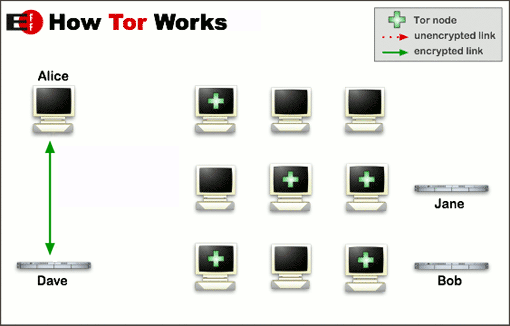
\includegraphics[width=9cm]{tor1}
    \end{center}
    \only<1>
    {
      Request listing of Tor nodes from Directory Authorities (DirAuths)
    }
    \only<2>
    {
    Pick entry, middle, and exit node; obtain their public keys from directory
    mirror (DirServ)
    }
  }
  \only<3>
  {
    \begin{center}
      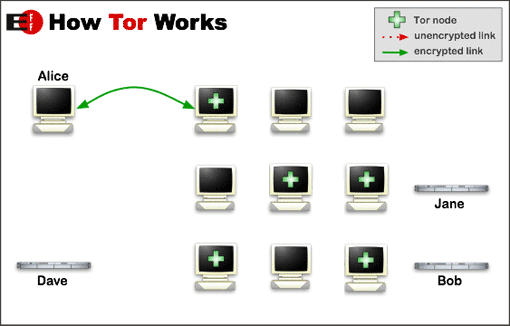
\includegraphics[width=9cm]{tor2}
    \end{center}
    Exchange symmetric key with entry node (Diffie-Hellman)
  }
  \only<4>
  {
    \begin{center}
      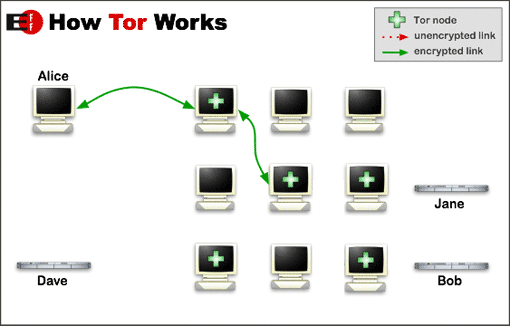
\includegraphics[width=9cm]{tor3}
    \end{center}
    Exchange key with middle node (tunnelled through entry node)
  }
  \only<5>
  {
    \begin{center}
      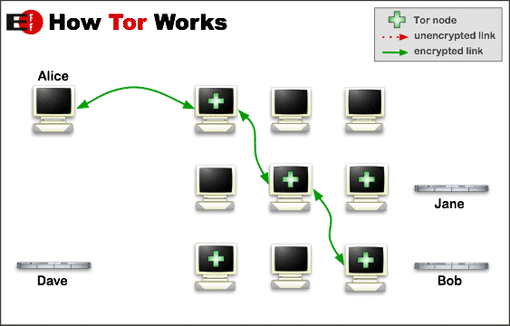
\includegraphics[width=9cm]{tor4}
    \end{center}
    Exchange key with exit node (tunnelled through middle node, tunnelled
    through entry node)
  }
  \only<6>
  {
    \begin{center}
      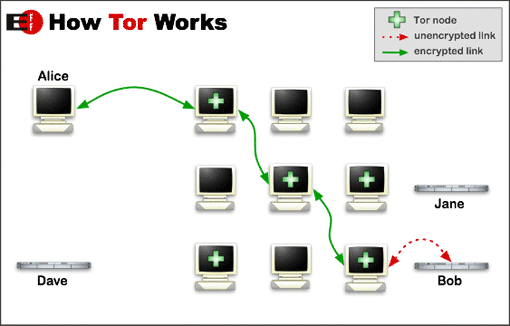
\includegraphics[width=9cm]{tor5}
    \end{center}
    Communicate with Bob (\texttt{theintercept.com})
  }
\end{frame}


\begin{frame}
  \frametitle{Some problems with Tor, part I}
  \begin{itemize} 
    \item Tor offers anonymity up to the transport layer
    \item <2-> Tor cannot offer application-level anonymity
    \item <2-> Example: I connect through Tor and send a tweet as \texttt{@isislovecruft}:\\[2mm]
      ``My name is Isis Agora Lovecruft, but my \emph{real} name is Urte
      Pfiffer, I'm 25-years-old, and my IP address is 106.187.37.158.''
    \item<3-> Various Bittorrent send the IP address as part of application data
    \item<3-> Conclusion:
      \href{https://blog.torproject.org/blog/bittorrent-over-tor-isnt-good-idea}{Bittorrent
        over Tor isn't a good idea} (It's also a bad idea for other reasons,
      e.g. the torrent bandwidth allocation algorithm doesn't play nicely with Tor)
    \item<4-> Browsers are easily identifiable, see
      \href{https://panopticlick.eff.org/index.php?action=log&js=yes}{Panopticlick
        by EFF}
    \item<4-> Conclusion: Use the
      \href{https://www.torproject.org/projects/torbrowser.html.en}{Tor browser}
      (modified Firefox)
    \item<5-> Tor re-uses an existing circuit for new TCP connections for 10
      minutes, but Tor Browser isolates (i.e. uses different) circuits, per
      second-level domain name in the URL bar.
    \item<6-> If you transparently proxy several applications through Tor
      simultaneously, and one leaks your IP address (bad apple attack), this
      activity may be linkable to the activity of other applications and
      decrease anonymity.
  \end{itemize} 
\end{frame}


\begin{frame}
  \frametitle{Some problems with Tor, part II}
  \begin{itemize}
    \item Most attacks in practice attempt, or assume, control of both the
      entry and exit (\emph{traffic confirmation attacks})
    \item<2-> Tor has a leaky-pipe topology, meaning that some types of commands
      and cells can be sent between relays in a circuit, not just from the user
      to the edge relay.
      \begin{itemize}
        \item<3-> This is how the recent CMU attack worked:
        \item<4-> Two
          \href{https://blog.torproject.org/blog/tor-security-advisory-relay-early-traffic-confirmation-attack/}{specific
            types of command} ($relay$ and $relay\_early$) are permitted to go
          down both the forward and reverse paths
        \item<5-> We fixed a bug ($\#1038$) where infinite-length circuits could
          be created (which allowed a \emph{resource-exhaustion attack}), by
          limiting the number of $relay\_early$s in the forward direction.
        \item<6-> We didn't limit the number of $relay\_early$s in the reverse
          direction, which allowed the CMU researchers to encode tags by
          alternating $relay$ and $relay\_early$ cells.
        \item<7-> CMU researchers simultaneously did a \emph{Sybil attack} by
          running several high-bandwidth relays in both entry and exit positions.
      \end{itemize}
  \end{itemize}
\end{frame}


\begin{frame}
  \frametitle{Correlation attacks}
  \begin{itemize}
    \item Tor is aiming at low latency (for web browsing etc.)
    \item Tor does not wait for traffic to do mixing
    \item<2-> \emph{Timing correlation attacks} are still theoretically possible:
      \begin{itemize}
        \item Think of the whole Tor network as one big proxy
        \item Correlate traffic going into and out of this proxy
      \end{itemize}
    \item<3-> Tor currently doesn't really do padding:
      \begin{itemize}
        \item There are patches for the upcoming (0.2.8) version to use padding
          in the outer TLS connection layer (not circuit-layer), in order to
          decrease the resolution of timing correlation attacks in netflow records.
        \item There are plans to implement adaptive padding techniques (see the
          \href{http://arxiv.org/pdf/1512.00524.pdf}{``WTF-PAD'' paper}) at the
          circuit-level in the future to defend against \emph{website traffic
            fingerprinting} correlation attacks.
      \end{itemize}
  \end{itemize}
\end{frame}


\begin{frame}
  \frametitle{NSA stinks}
  \begin{itemize}
    \item Snowden leaked NSA slides ``Tor stinks'' from 2007
    \item Quotes from these slides:\\[4mm]
      \emph{``We will never be able to de-anonymize all Tor users all the time.''}\\[4mm]
      \emph{``With manual analysis we can de-anonymize a \textbf{\underline{very small fraction}} of Tor users, 
      however \textbf{\underline{no}} success de-anonymizing a user in response to a TOPI request/on demand.''}
    \item<2-> Our assumption is that they meant they were sometimes able to
      control both the entry and exit relays for some circuits (but couldn't do
      it on demand), however that they otherwise cannot deanonymise users.
    \item<3-> Not-so-secretly, we think the NSA stinks too. :P
  \end{itemize}
\end{frame}


\begin{frame}
  \frametitle{Tor as censorship circumvention}
  \begin{itemize}
    \item Various countries filter Internet traffic by destination address
    \item Most prominent example: Great Firewall of China
    \item<2-> Firewalls and gateways cannot see the true destination of Tor traffic
    \item<2-> Tor is a powerful tool to circumvent online censorship (e.g., in China,
      Iran, Turkey, Kazakhstan, Ethiopia, others)
    \item<3-> Can also use Tor to circumvent country filters:
      \begin{itemize}
      \item Need an IP address that isn't in Germany (e.g. because of GEMA
        restrictions on YouTube): can use Tor access YouTube from a non-German
        IP address.
      \end{itemize}
  \end{itemize}
\end{frame}


\begin{frame}
  \frametitle{Censorship of Tor}
  \begin{itemize}
    \item Easy solution for censors: 
      \begin{itemize}
        \item<2-> Obtain list of Tor nodes from the Directory Authorities
        \item<3-> Block access to the Tor network (all relays)
      \end{itemize}
    \item<4-> Solution: Tor Bridges
  \end{itemize}
\end{frame}

\begin{frame}
  \frametitle{Tor Bridges}

  \begin{itemize}
  \item \emph{Bridge relays} or \emph{bridges} are secret entrances to the Tor
    network.
  \item<2-> Bridge IP address and other connection information must be
    distributed out-of-band
  \item<3-> DPI or an active adversary is required to identify Bridges
  \item<4-> Distributed via a centralised system called BridgeDB. Users can
    currently obtain bridges by:
      \begin{itemize}
        \item visiting \url{https://bridges.torproject.org/}
        \item writing e-mail to \href{mailto:bridges@torproject.org}{bridges@torproject.org}
      \end{itemize}
  \item<5-> Yes, that whole system sucks.  One of my current projects is
    redesigning and rewriting it.
  \end{itemize}
\end{frame}


\begin{frame}
  \frametitle{Pluggable Transports}
  \begin{itemize}
    \item Censors can also block Tor by identifying Tor traffic
    \item<2-> Tor traffic is relatively easy to identify:
      \begin{itemize}
        \item Disguised as HTTPS traffic, but
        \item uses random domain names 
        \item has a characteristic packet-size distribution
      \end{itemize}
    \item<3-> Solution: disguise Tor traffic as other traffic
    \item<3->
      \href{https://www.torproject.org/docs/pluggable-transports.html.en}{Pluggable
        Transport API} allows communication between obfuscating SOCKS proxy and
      Tor client
  \end{itemize}
\end{frame}


\begin{frame}[plain]
  \begin{center}
    \href{https://www.torproject.org/docs/tor-doc-relay.html.en}
    {
\includegraphics[width=6cm]{runtor}}
  \end{center}
\end{frame}


\end{document}
